% !TeX root = ../../../main.tex
\begin{figure}[!ht]

\centering
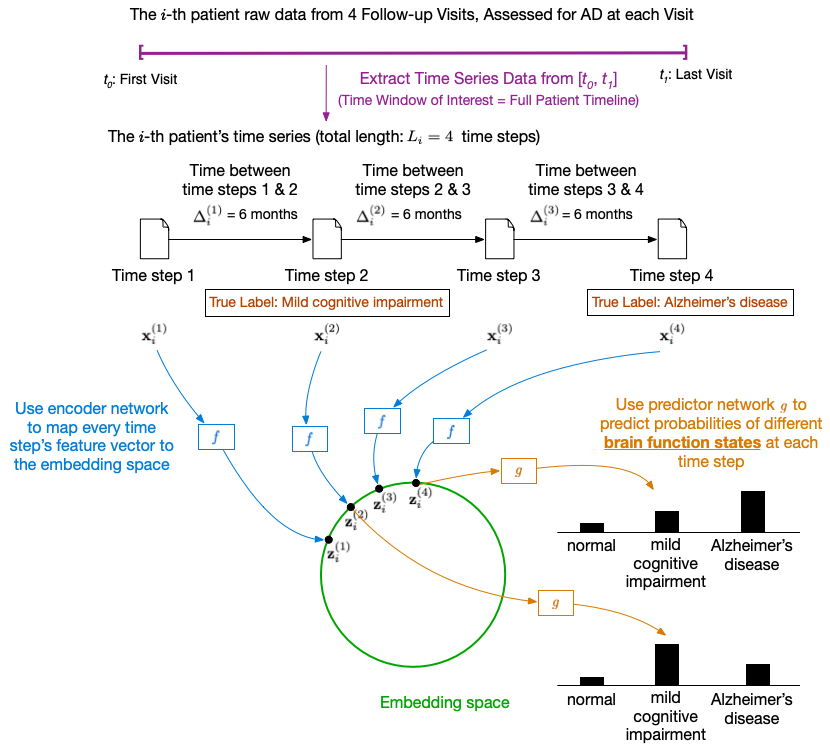
\includegraphics[width=.99\linewidth]{Appendices/appendix-ch02/images/ADNI-Setup.png}
%\vspace{-2.5em}
 \caption{Setup for ADNI Experiment at Inference time from \ChTwoSmallCaps{Temporal-SCL}: First, we extract time series data for each patient from their complete timeline of available data spanning all the 6-month follow-up visits. This time series data maintains the same 6-month interval time steps as the raw data, with each time step having its own true class label representing one of the three possible brain function states. The resulting time series will have its features at each time step mapped onto the embedding space learned by our encoder. Subsequently, these resulting embeddings will be passed through our predictor network to predict the brain function class of each patient at every time step.
 %\vspace{-1em}
 }   \ChTwoFloatLabel{ch02:fig:adni-setup}
\end{figure}